\documentclass[tikz, border=10pt]{standalone}
\usepackage{iftex}
\ifluatex
  \usepackage{fontspec}
  \usepackage{unicode-math}
  \setmainfont{Fira Sans}
  \setmonofont{Fira Mono}
  \setmathfont{Fira Math}
  % Fallback only for set-difference glyphs missing in Fira Math.
  \setmathfont{STIX Two Math}[range={"29F5,"2216}]
\else
  \usepackage[T1]{fontenc}
\fi

\usepackage{amsmath}
\usepackage{tikz}
\usetikzlibrary{arrows.meta}
\tikzset{every node/.style={font=\Large}}

% Theme toggle: set \darkbgfalse for light background preview.
\newif\ifdarkbg
\darkbgfalse % uncomment for light background
\ifdarkbg
  \colorlet{axiscol}{white}
  \colorlet{gridcol}{white!30!black}
  \colorlet{ticklabelcol}{white}
  \colorlet{funcol}{yellow!85!white}
\else
  \colorlet{axiscol}{black}
  \colorlet{gridcol}{black!25!white}
  \colorlet{ticklabelcol}{black}
  \colorlet{funcol}{blue!70!black}
\fi

\begin{document}
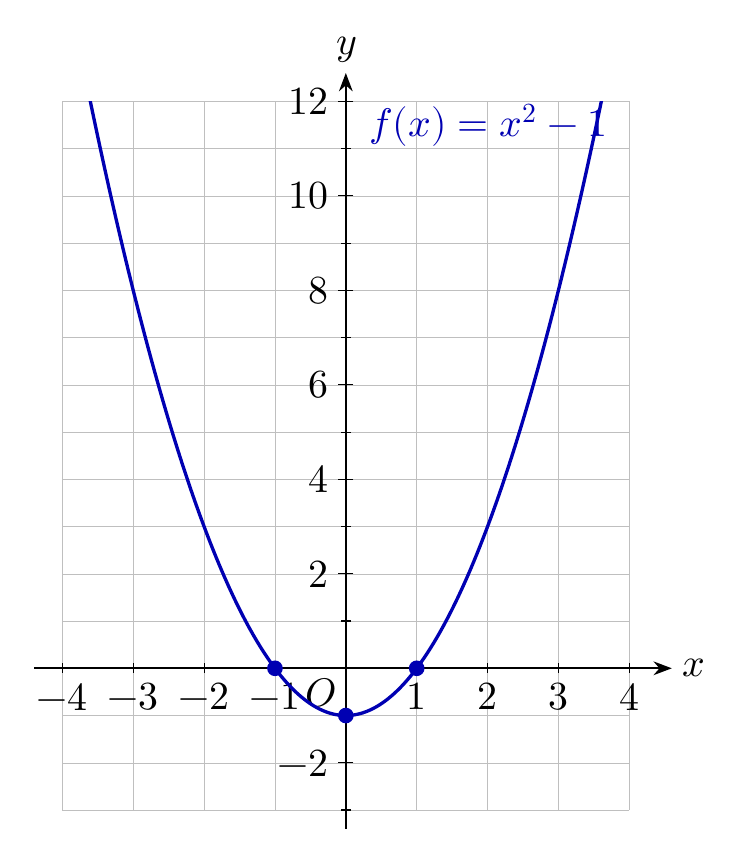
\begin{tikzpicture}[xscale=0.9, yscale=0.6, >=Stealth]

  % Cartesian grid.
  \draw[step=1, very thin, gridcol] (-4,-3) grid (4,12);

  % Axes.
  \draw[->, thick, axiscol] (-4.4,0) -- (4.6,0)
    node[right, text=axiscol] {$x$};
  \draw[->, thick, axiscol] (0,-3.4) -- (0,12.6)
    node[above, text=axiscol] {$y$};

  % Tick marks — x axis.
  \foreach \x in {-4,-3,-2,-1,1,2,3,4} {
    \draw[axiscol] (\x, 3pt) -- (\x, -3pt)
      node[below, text=ticklabelcol] {$\x$};
  }

  % Tick marks — y axis (labelled every 2, minor every 1).
  \foreach \y in {-2,2,4,6,8,10,12} {
    \draw[axiscol] (3pt,\y) -- (-3pt,\y)
      node[left, text=ticklabelcol] {$\y$};
  }
  \foreach \y in {-3,-1,1,3,5,7,9,11} {
    \draw[axiscol] (2pt,\y) -- (-2pt,\y);
  }

  % Origin label.
  \node[below left, text=axiscol] at (0,0) {$O$};

  % Function curve: f(x) = x² − 1, clipped to the plot window.
  \begin{scope}
    \clip (-4,-3) rectangle (4,12);
    \draw[domain=-4:4, smooth, very thick, funcol, samples=120]
      plot (\x, {(\x)^2 - 1});
  \end{scope}

  % Function label.
  \node[right, text=funcol] at (0.2,11.5) {$f(x)=x^2-1$};

  % Vertex.
  \node[circle, fill=funcol, inner sep=2pt] at (0,-1) {};
  % \node[right, text=funcol] at (0.15,-1) {$(0,-1)$};

  % x-intercepts.
  \node[circle, fill=funcol, inner sep=2pt] at (-1,0) {};
    % node[above left, text=funcol] {$(-1,0)$};
  \node[circle, fill=funcol, inner sep=2pt] at (1,0) {};
    % node[above right, text=funcol] {$(1,0)$};

\end{tikzpicture}
\end{document}
